\chapter{Experimentální část}
Tato kapitola prezentuje vyhodnocení implementovaných optimalizačních metod na dvojici instancí TSPLIB \texttt{a280} (symetrická) a \texttt{kro124p} (asymetrická). Cílem je porovnat kvalitu nalezeného řešení, stabilitu heuristik a metaheuristik, konvergenční chování i kompromis mezi výpočetním časem a dosaženou odchylkou od optima ve dvou odlišných typech úloh.

\section{Nastavení experimentu}
\label{sec:exp_setup}
Měření bylo provedeno nad instancemi \texttt{a280} a \texttt{kro124p}. Testovaná sada algoritmů obsahuje metody 2-opt, 3-opt, LK, LKH, GA, ACO, RSO a SA a jejich parametrizace byla převzata z ladění pomocí knihovny \texttt{Optuna}. Všechny heuristiky i metaheuristiky byly v rámci jednotného protokolu vyhodnoceny ve 30 bězích, aby bylo možné konzistentně posoudit stabilitu i rozptyl výsledků.

Každý běh byl řízen pevným master seedem, z něhož se odvozovaly seed hodnoty pro jednotlivé algoritmy a opakování, takže experiment je reprodukovatelný a porovnání mezi metodami zůstává férové napříč oběma instancemi. U deterministických metod tímto postupem nevzniká variabilita řešení, ale zachovává se jednotný experimentální režim a stejná reportovací logika.

V závěrečné fázi byl každý algoritmus doplněn lokálním vylepšením trasy, aby výsledná hodnota reprezentovala nejen hrubý výstup hlavní heuristiky, ale i běžnou praktickou finalizaci řešení. U symetrické instance byl tento krok realizován především pomocí 2-opt zlepšování, zatímco u asymetrické instance byl použit lokální průchod bez reverzace segmentů založený na operátorech \emph{swap}, \emph{relocate} a \emph{or-opt}, které zachovávají orientaci hran. Metody 2-opt, 3-opt a LK jsou v této implementaci navrženy pro symetrické TSP a na asymetrické instanci nejsou nasazovány, protože jejich klasické kroky založené na reverzaci segmentu nejsou pro orientované hrany přímo použitelné.

Instance \texttt{a280} a \texttt{kro124p} byly zvoleny záměrně, protože společně pokrývají dva odlišné charaktery úlohy a umožňují sledovat, jak se stejné algoritmické principy chovají v symetrickém i asymetrickém prostředí. Současně jde o velikosti, které jsou dostatečně náročné pro vznik měřitelných rozdílů mezi metodami, ale stále výpočetně zvládnutelné při zachování 30 opakování pro každou metodu.

\section{Konvergenční průběhy metaheuristik}
\label{sec:exp_convergence}
Konvergenční chování je hodnoceno samostatně pro obě instance. Osa \(x\) v grafech představuje normalizovaný průběh iterací od začátku do konce běhu a osa \(y\) odchylku od referenčního optima v procentech.

\subsection{Symetrická instance \texttt{a280}}
Na instanci \texttt{a280} je patrné, že všechny metaheuristiky dosahují nejvýraznějšího zlepšení v úvodní fázi běhu a následně přecházejí do jemnějšího dolaďování. Konvergenční průběhy ACO \ref{fig:conv_aco_a280} a GA \ref{fig:conv_ga_a280} jsou stabilnější než SA \ref{fig:conv_sa_a280}, která má širší rozptyl trajektorií, a RSO \ref{fig:conv_rso_a280} se obvykle drží ve středním pásmu mezi robustností a kvalitou finálního řešení.

\begin{figure}[H]
    \centering
    
\includegraphics[width=\textwidth]{Figures/symmetric_a280/convergence_spaghetti_ACO.png}
    \caption{Konvergenční průběhy ACO pro instanci \texttt{a280}}
    \label{fig:conv_aco_a280}
\end{figure}

\begin{figure}[H]
    \centering
    
\includegraphics[width=\textwidth]{Figures/symmetric_a280/convergence_spaghetti_GA.png}
    \caption{Konvergenční průběhy GA pro instanci \texttt{a280}}
    \label{fig:conv_ga_a280}
\end{figure}

\begin{figure}[H]
    \centering
    
\includegraphics[width=\textwidth]{Figures/symmetric_a280/convergence_spaghetti_RSO.png}
    \caption{Konvergenční průběhy RSO pro instanci \texttt{a280}}
    \label{fig:conv_rso_a280}
\end{figure}

\begin{figure}[H]
    \centering
    
\includegraphics[width=\textwidth]{Figures/symmetric_a280/convergence_spaghetti_SA.png}
    \caption{Konvergenční průběhy SA pro instanci \texttt{a280}}
    \label{fig:conv_sa_a280}
\end{figure}

\subsection{Asymetrická instance \texttt{kro124p}}
Na instanci \texttt{kro124p} zůstává průběh analogický v tom, že největší část zlepšení probíhá na začátku běhu, ale rozdíly mezi metodami jsou více ovlivněny asymetrií hran a volbou ATSP-safe sousedství. Konvergenční průběhy ACO \ref{fig:conv_aco_kro124p}, GA \ref{fig:conv_ga_kro124p}, RSO \ref{fig:conv_rso_kro124p} a SA \ref{fig:conv_sa_kro124p} potvrzují, že metody lépe využívající kombinaci \emph{swap}/\emph{relocate}/\emph{or-opt} mají obvykle vyšší stabilitu než přístupy citlivé na počáteční trajektorii.

\begin{figure}[H]
    \centering
    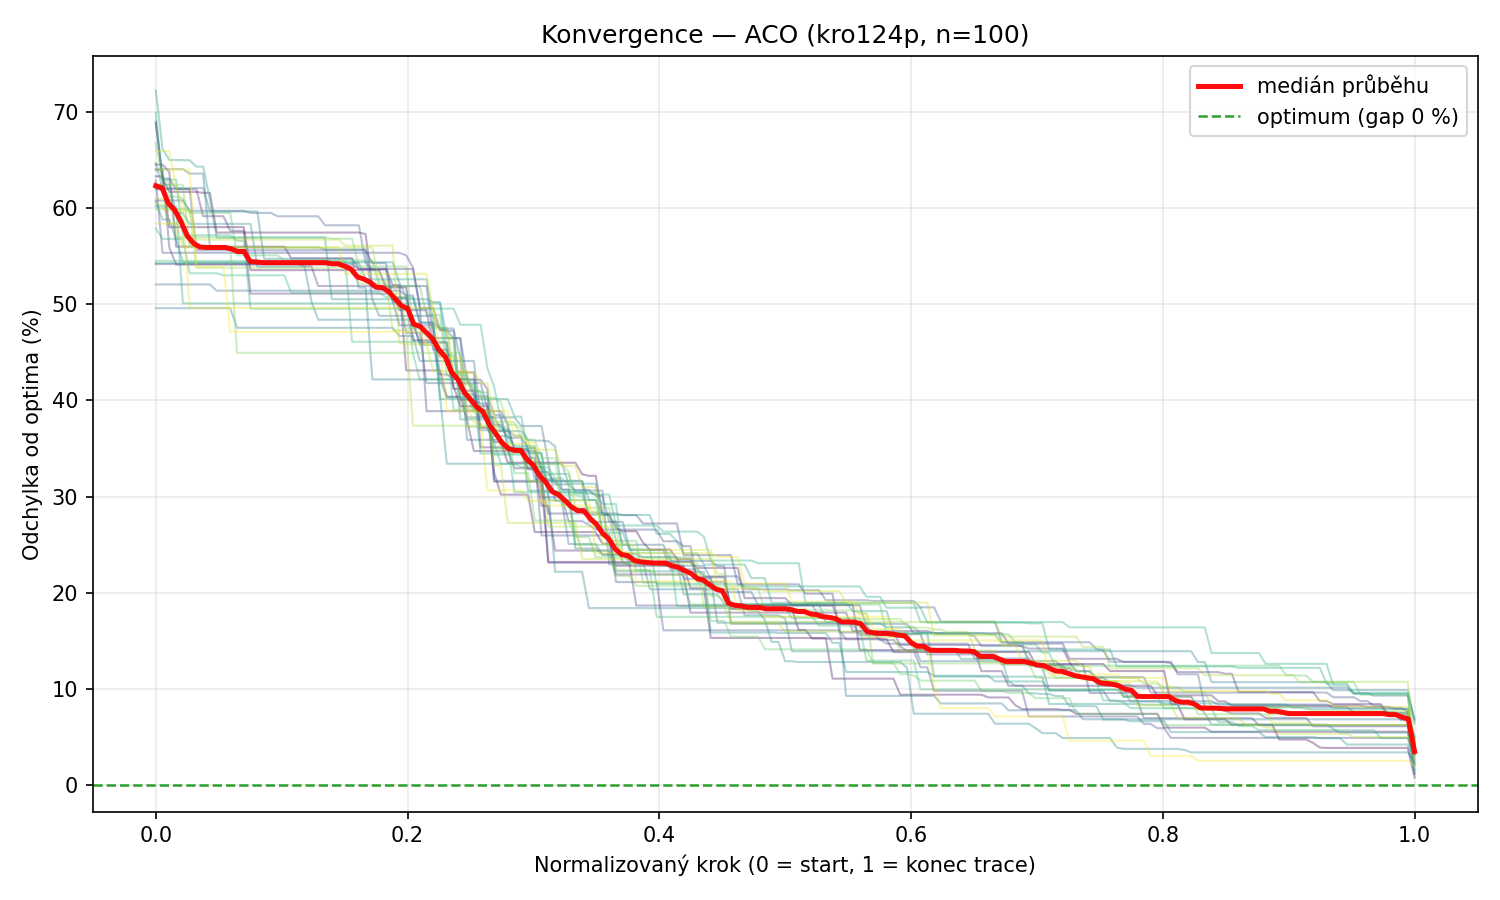
\includegraphics[width=\textwidth]{Figures/asymmetric_kro124p/convergence_spaghetti_ACO.png}
    \caption{Konvergenční průběhy ACO pro instanci \texttt{kro124p}}
    \label{fig:conv_aco_kro124p}
\end{figure}

\begin{figure}[H]
    \centering
    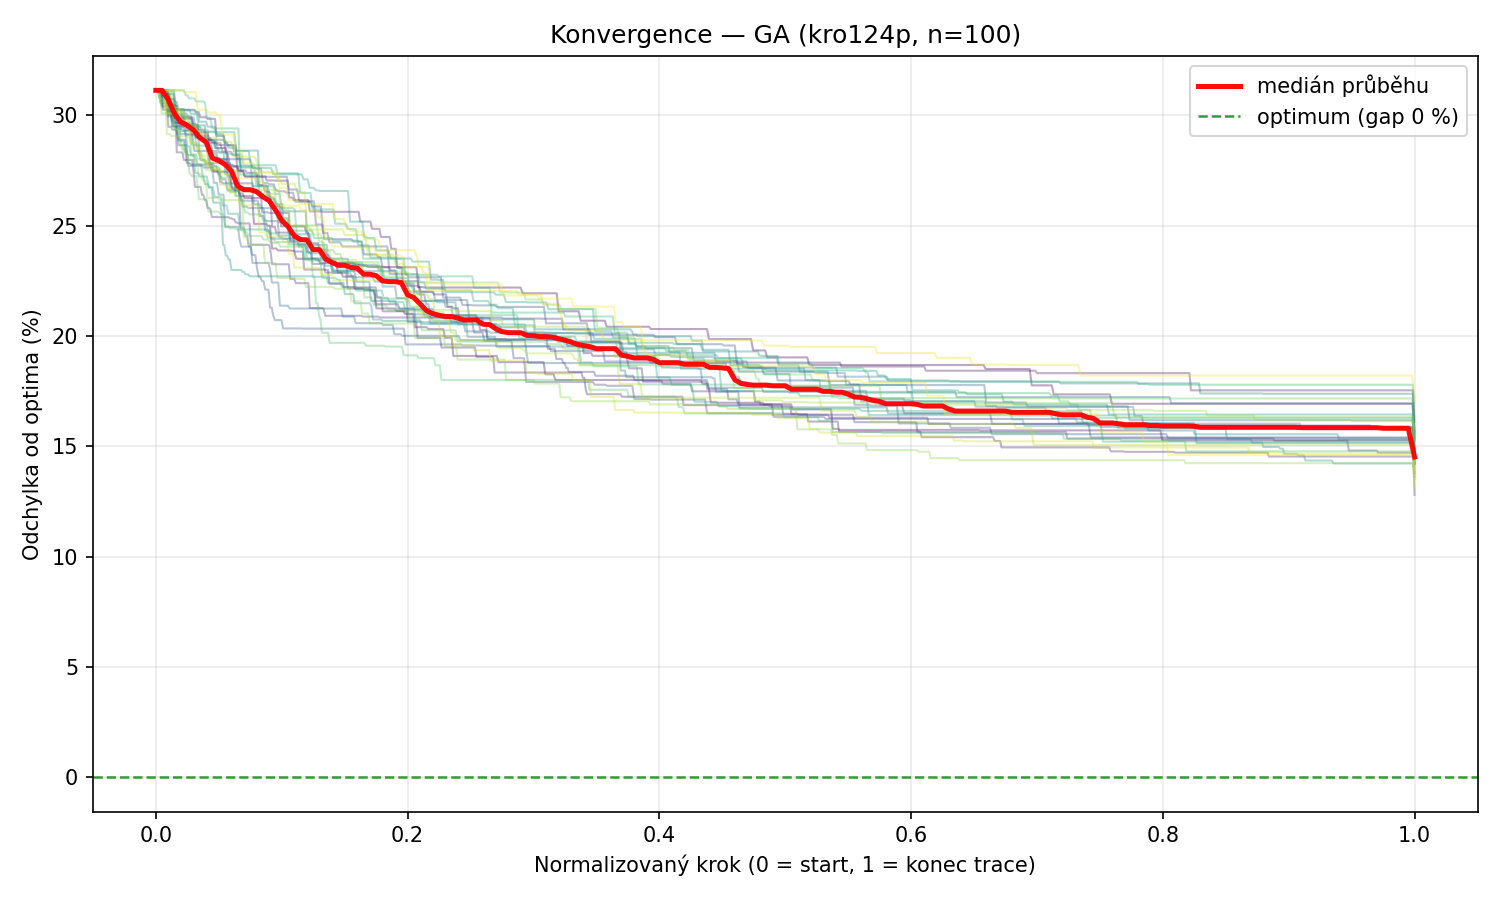
\includegraphics[width=\textwidth]{Figures/asymmetric_kro124p/convergence_spaghetti_GA.png}
    \caption{Konvergenční průběhy GA pro instanci \texttt{kro124p}}
    \label{fig:conv_ga_kro124p}
\end{figure}

\begin{figure}[H]
    \centering
    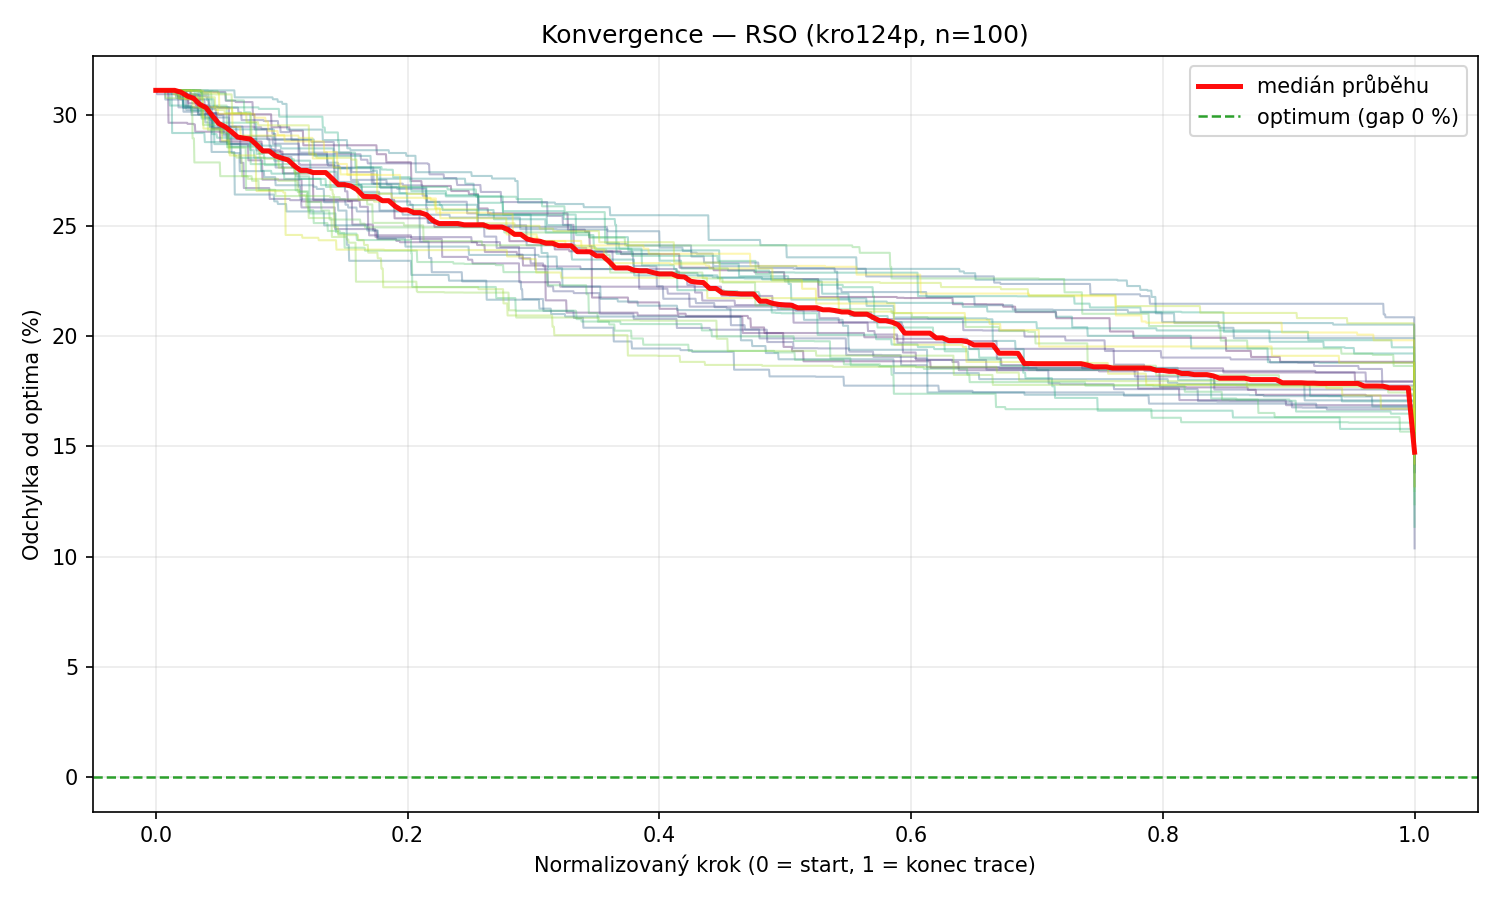
\includegraphics[width=\textwidth]{Figures/asymmetric_kro124p/convergence_spaghetti_RSO.png}
    \caption{Konvergenční průběhy RSO pro instanci \texttt{kro124p}}
    \label{fig:conv_rso_kro124p}
\end{figure}

\begin{figure}[H]
    \centering
    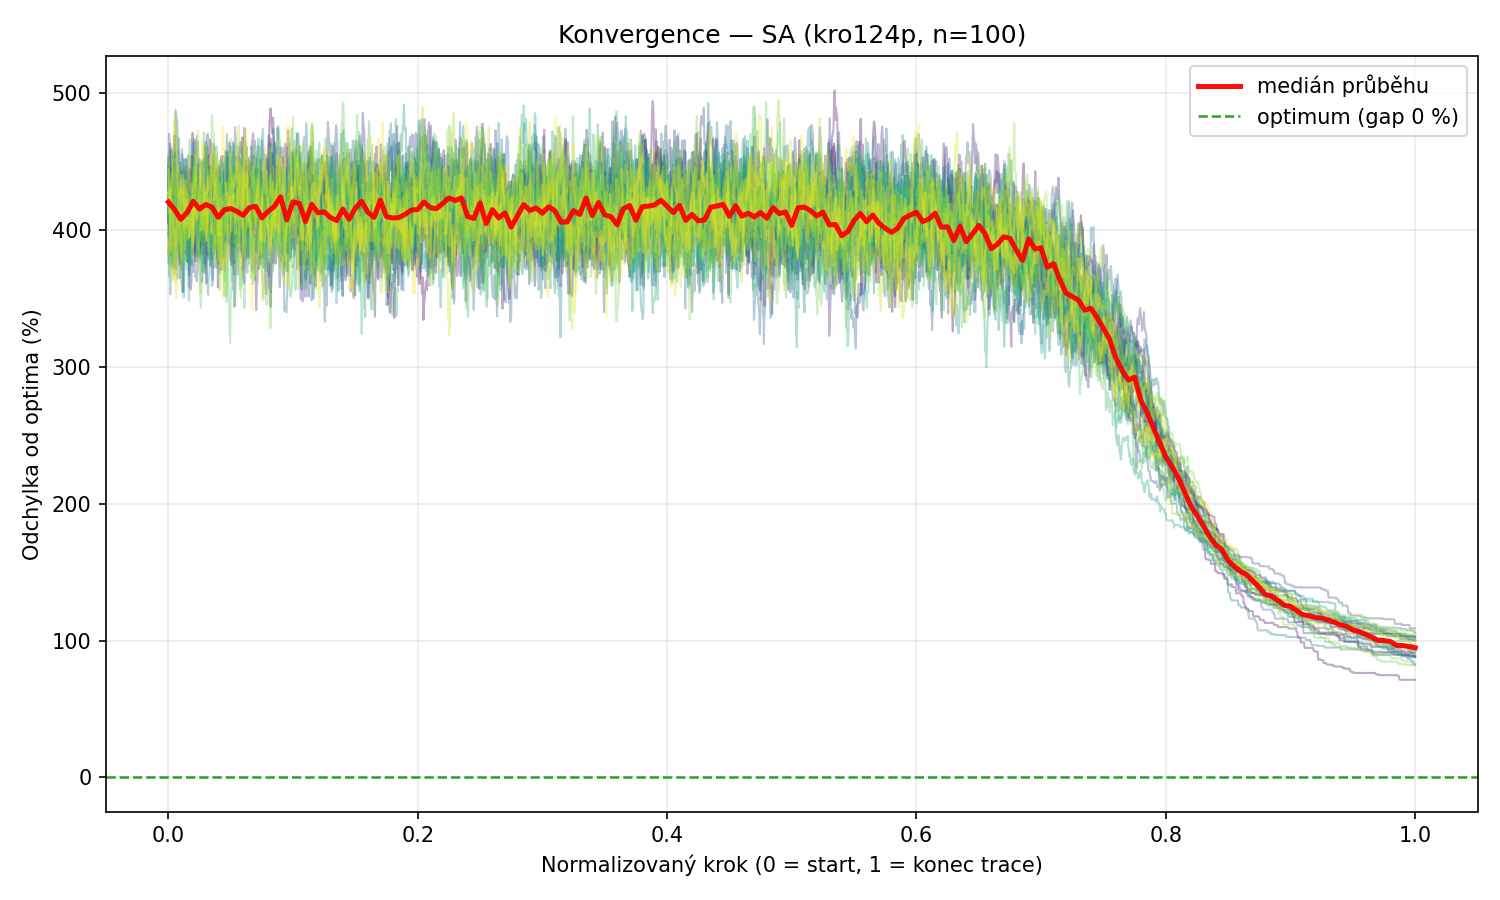
\includegraphics[width=\textwidth]{Figures/asymmetric_kro124p/convergence_spaghetti_SA.png}
    \caption{Konvergenční průběhy SA pro instanci \texttt{kro124p}}
    \label{fig:conv_sa_kro124p}
\end{figure}

\section{Rozdělení kvality řešení a statistická významnost}
\label{sec:exp_distribution}
Rozdělení výsledků stochastických metod je opět uvedeno odděleně pro symetrickou a asymetrickou instanci, aby bylo možné přesně odlišit vliv typu úlohy od vlivu samotného algoritmu.

\subsection{Symetrická instance \texttt{a280}}
Na instanci \texttt{a280} je v boxplotu \ref{fig:boxplots_meta_a280} nejdříve patrné ostré rozdělení na dvě výkonnostní skupiny. ACO, GA a RSO drží délky tras v relativně úzkém pásmu nad referenčním optimem (v grafu vyznačeným zelenou vodorovnou čárou): ACO má nejnižší medián i střední hodnotu (obě zhruba kolem \(2{,}75\cdot 10^3\)) a současně nejlepší spodní hranici rozptylu, takže i horší běhy zůstávají blíže optimu než u GA a RSO. GA a RSO mají podobně úzké krabice a krátké vousy, což ukazuje na vysokou opakovatelnost výsledku napříč 30 běhy; GA je v mediánu mírně lepší než RSO (řádově o desítky jednotek délky). Naproti tomu SA koncentruje výsledky výrazně výše (medián zhruba kolem \(3{,}5\cdot 10^3\)) a má širší krabici, takže na této instanci a při použité parametrizaci nedosahuje kvality srovnatelné s ostatními metaheuristikami.

Houslový graf se stripplotem \ref{fig:violin_meta_a280} stejný obraz doplňuje o tvar rozdělení a o jednotlivé realizace běhů. U ACO je vidět, že hustota není nejužší, ale je posunutá k nejnižším délkám a stripové body sahají do nejlepších hodnot v celém souboru měření; praktický závěr je, že ACO častěji nachází velmi dobré trasy, i když variabilita mezi běhy není minimální. U GA a RSO jsou body těsně seskupené kolem vlastního mediánu, což potvrzuje stabilní, málo kolísavý výkon bez extrémně špatných výkyvů. U SA se všechny body nacházejí v odděleném pásmu bez překryvu s ostatními metodami, takže rozdíl není jen průměrný efekt, ale platí pro každý zaznamenaný běh.

AutoRank (CD diagram) \ref{fig:autorank_frequentist_a280} shrnuje pořadí metod podle průměrných řádů napříč synchronními opakováními (stejný \texttt{run\_index} pro všechny metaheuristiky) a tlusté spojnice označují páry algoritmů, u nichž post-hoc test po Friedmanově hodnocení neshledal statisticky významný rozdíl na hladině \(p = 0{,}05\). ACO má nejlepší průměrný řád a v diagramu nemá spojnici s žádnou z ostatních metod, takže je na \texttt{a280} statisticky významně lepší než GA, RSO i SA. GA a RSO jsou v diagramu spojeny, takže rozdíl pozorovaný v boxplotu sice naznačuje mírnou výhodu GA, ale v tomto párovém experimentálním uspořádání nelze jednostranně tvrdit statisticky prokázanou převahu jedné z nich nad druhou. SA zůstává izolovaně na nejhorším řádu a je významně horší než všechny ostatní testované metaheuristiky.

\begin{figure}[H]
    \centering
    
\includegraphics[width=\textwidth]{Figures/symmetric_a280/boxplots_metaheuristics.png}
    \caption{Boxplot rozdělení odchylek metaheuristik pro instanci \texttt{a280}}
    \label{fig:boxplots_meta_a280}
\end{figure}

\begin{figure}[H]
    \centering
    
\includegraphics[width=\textwidth]{Figures/symmetric_a280/violin_metaheuristics_strip.png}
    \caption{Houslový graf rozdělení odchylek metaheuristik pro instanci \texttt{a280}}
    \label{fig:violin_meta_a280}
\end{figure}

\begin{figure}[H]
    \centering
    
\includegraphics[width=0.95\textwidth]{Figures/symmetric_a280/autorank_plot_frequentist.png}
    \caption{Statistické srovnání metod pomocí autorank pro instanci \texttt{a280}}
    \label{fig:autorank_frequentist_a280}
\end{figure}

\subsection{Asymetrická instance \texttt{kro124p}}
Na \texttt{kro124p} se distribuce výsledků mění v návaznosti na orientované náklady hran, takže statistická významnost rozdílů odráží nejen kvalitu metaheuristiky jako takové, ale i její schopnost pracovat s asymetrickým sousedstvím. Boxplot \ref{fig:boxplots_meta_kro124p} a houslový graf \ref{fig:violin_meta_kro124p} ukazují rozptyl výsledků, zatímco Autorank \ref{fig:autorank_frequentist_kro124p} slouží jako kontrola toho, zda pozorované rozdíly představují stabilní trend, nebo pouze důsledek náhodného rozptylu.

\begin{figure}[H]
    \centering
    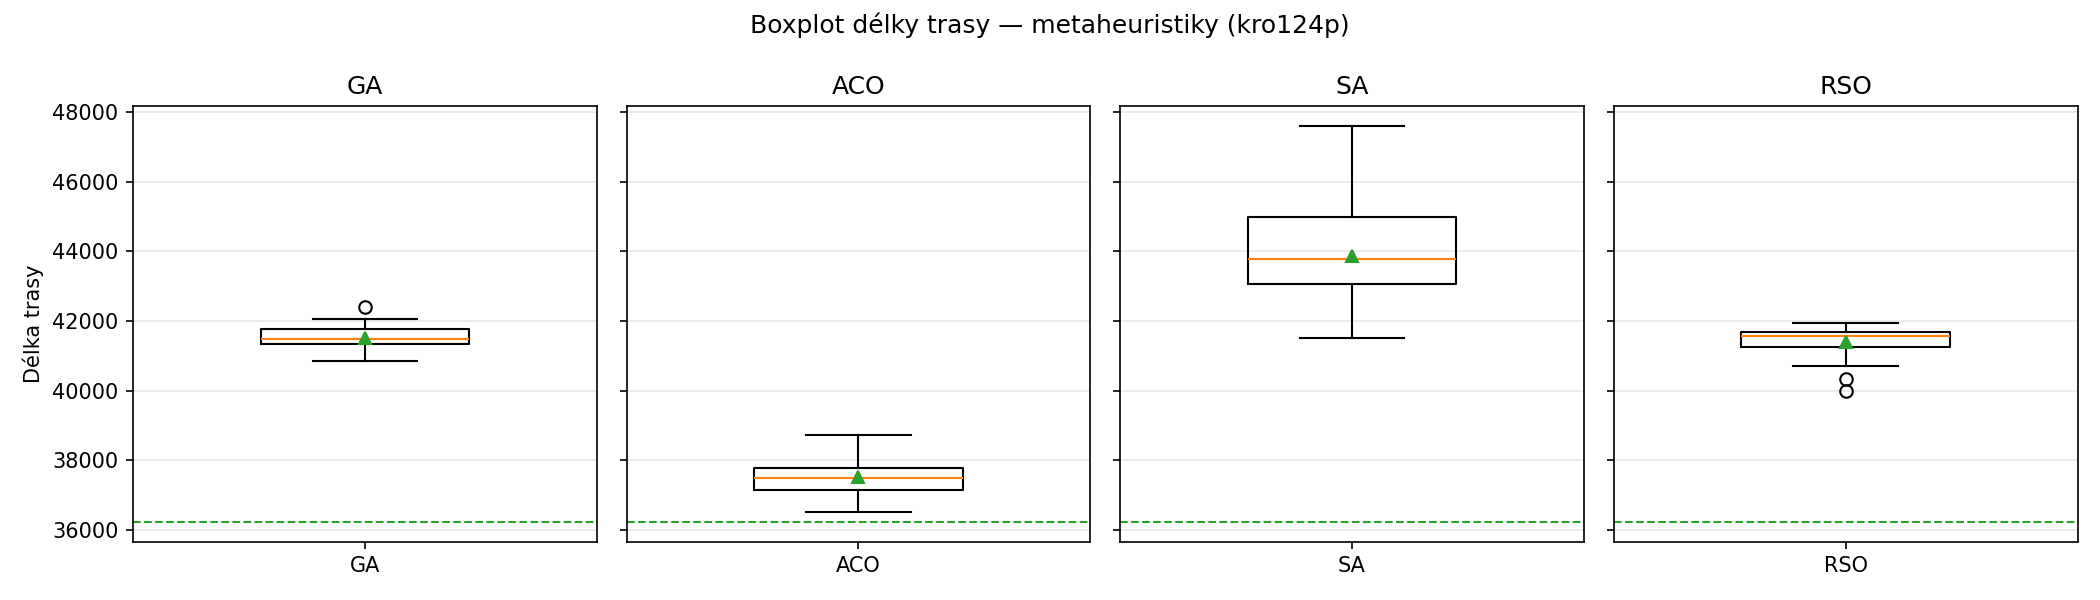
\includegraphics[width=\textwidth]{Figures/asymmetric_kro124p/boxplots_metaheuristics.png}
    \caption{Boxplot rozdělení odchylek metaheuristik pro instanci \texttt{kro124p}}
    \label{fig:boxplots_meta_kro124p}
\end{figure}

\begin{figure}[H]
    \centering
    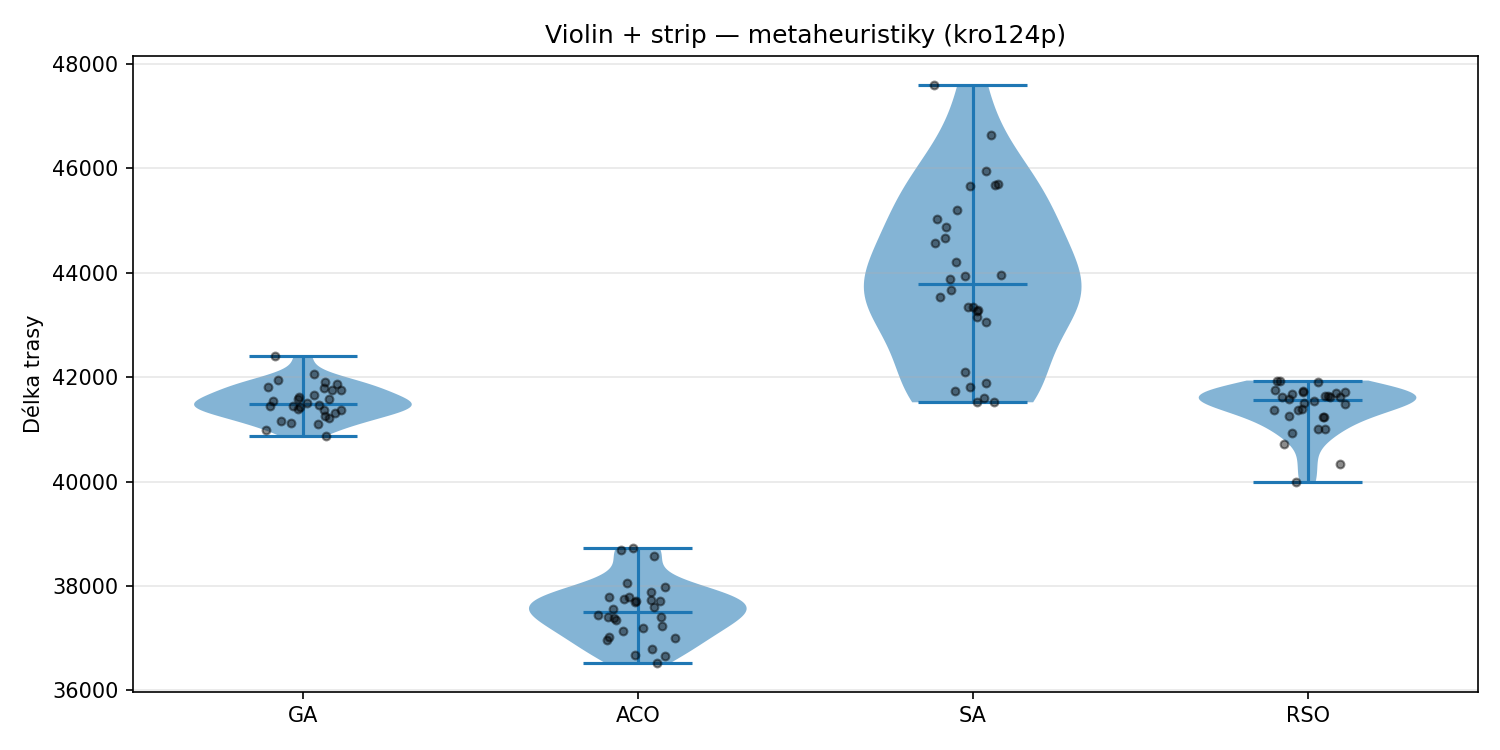
\includegraphics[width=\textwidth]{Figures/asymmetric_kro124p/violin_metaheuristics_strip.png}
    \caption{Houslový graf rozdělení odchylek metaheuristik pro instanci \texttt{kro124p}}
    \label{fig:violin_meta_kro124p}
\end{figure}

\begin{figure}[H]
    \centering
    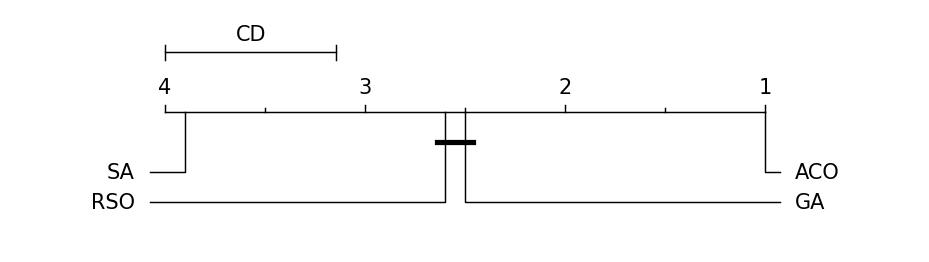
\includegraphics[width=0.95\textwidth]{Figures/asymmetric_kro124p/autorank_plot_frequentist.png}
    \caption{Statistické srovnání metod pomocí autorank pro instanci \texttt{kro124p}}
    \label{fig:autorank_frequentist_kro124p}
\end{figure}

\section{Globální srovnání všech metod}
\label{sec:exp_global}
Komplexní porovnání všech metod je uvedeno samostatně pro obě instance pomocí grafu kompromisu čas versus kvalita a souhrnné tabulky statistik.

\subsection{Symetrická instance \texttt{a280}}
Scatter graf \ref{fig:scatter_time_vs_gap_a280} umožňuje na instanci \texttt{a280} číst výsledky ve dvou dimenzích současně: na horizontální ose je výpočetní čas a na vertikální ose relativní odchylka od optima. Metody umístěné blíže levému dolnímu rohu proto představují nejvýhodnější kompromis, protože dosahují nízké chyby při současně nízké časové náročnosti. Rozptýlení bodů navíc ukazuje, zda je daný algoritmus stabilní napříč opakováními, nebo zda jeho výkon výrazně kolísá mezi jednotlivými běhy. Souhrnná tabulka \ref{fig:summary_table_optimum_vs_stats_a280} tento grafický pohled rozšiřuje o konkrétní statistiky (minimum, medián, průměr, směrodatná odchylka a nejlepší dosažená hodnota), což umožňuje přesněji oddělit algoritmy s konzistentně dobrým výkonem od metod, které dosáhnou kvalitního řešení jen v části běhů.

\begin{figure}[H]
    \centering
    
\includegraphics[width=0.95\textwidth]{Figures/symmetric_a280/scatter_time_vs_gap.png}
    \caption{Kompromis mezi časem výpočtu a odchylkou od optima pro instanci \texttt{a280}}
    \label{fig:scatter_time_vs_gap_a280}
\end{figure}

\begin{figure}[H]
    \centering
    
\includegraphics[width=\textwidth]{Figures/symmetric_a280/summary_table_optimum_vs_stats.png}
    \caption{Souhrnná tabulka výsledků pro instanci \texttt{a280}}
    \label{fig:summary_table_optimum_vs_stats_a280}
\end{figure}

\subsection{Asymetrická instance \texttt{kro124p}}
U instance \texttt{kro124p} je dvojici pohledů přiřazena role ověřit, jak se mění pořadí a stabilita metod v asymetrickém režimu. Scatter graf \ref{fig:scatter_time_vs_gap_kro124p} vyjadřuje časovou cenu dosažené přesnosti a souhrnná tabulka \ref{fig:summary_table_optimum_vs_stats_kro124p} uzavírá porovnání numerickým přehledem.

\begin{figure}[H]
    \centering
    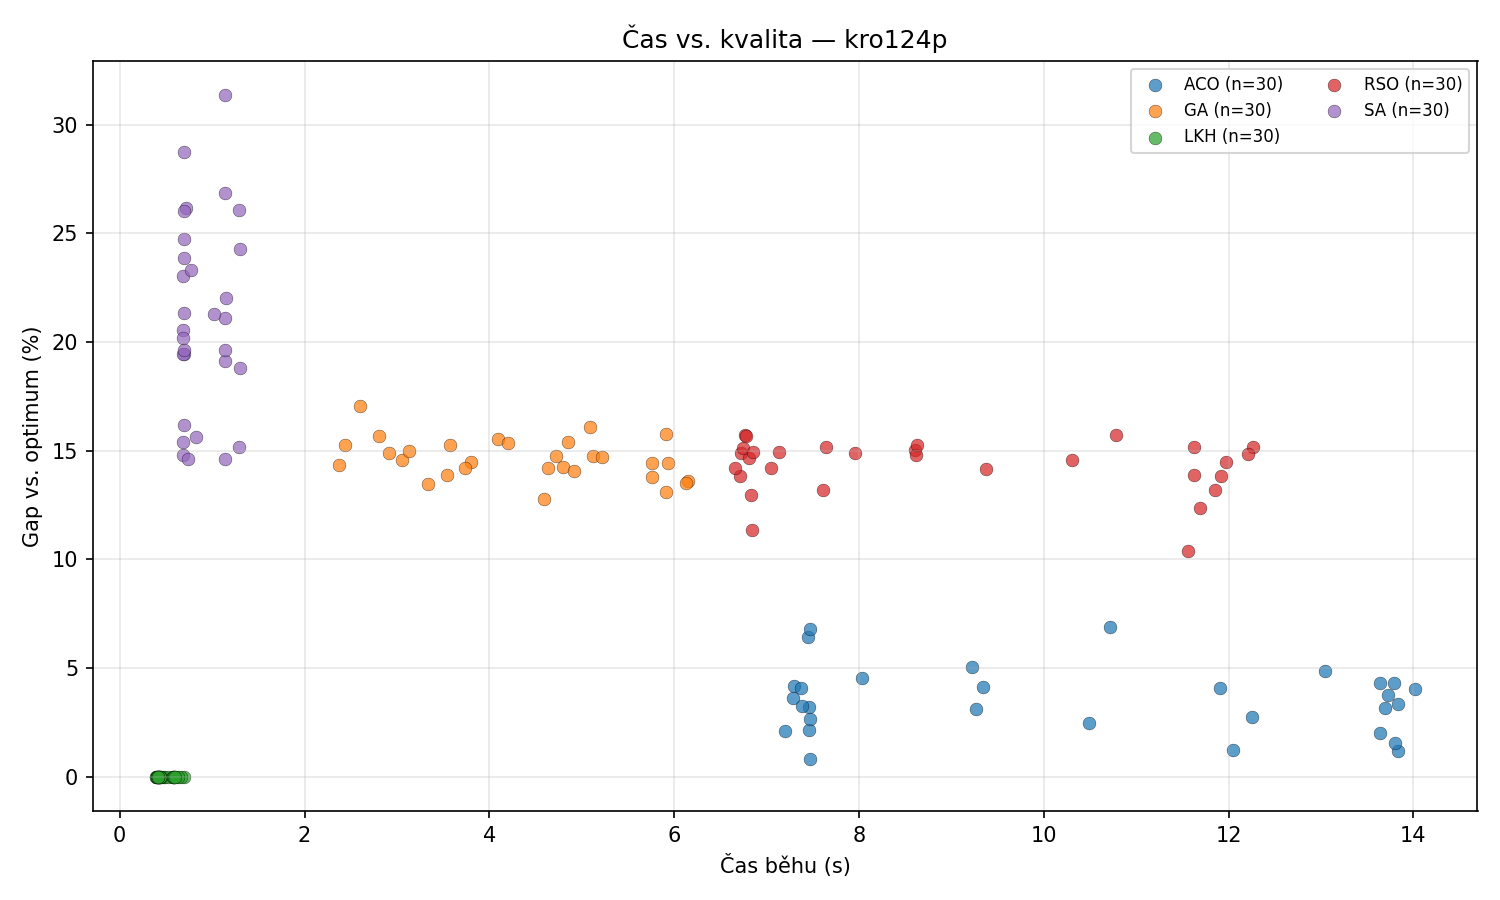
\includegraphics[width=0.95\textwidth]{Figures/asymmetric_kro124p/scatter_time_vs_gap.png}
    \caption{Kompromis mezi časem výpočtu a odchylkou od optima pro instanci \texttt{kro124p}}
    \label{fig:scatter_time_vs_gap_kro124p}
\end{figure}

\begin{figure}[H]
    \centering
    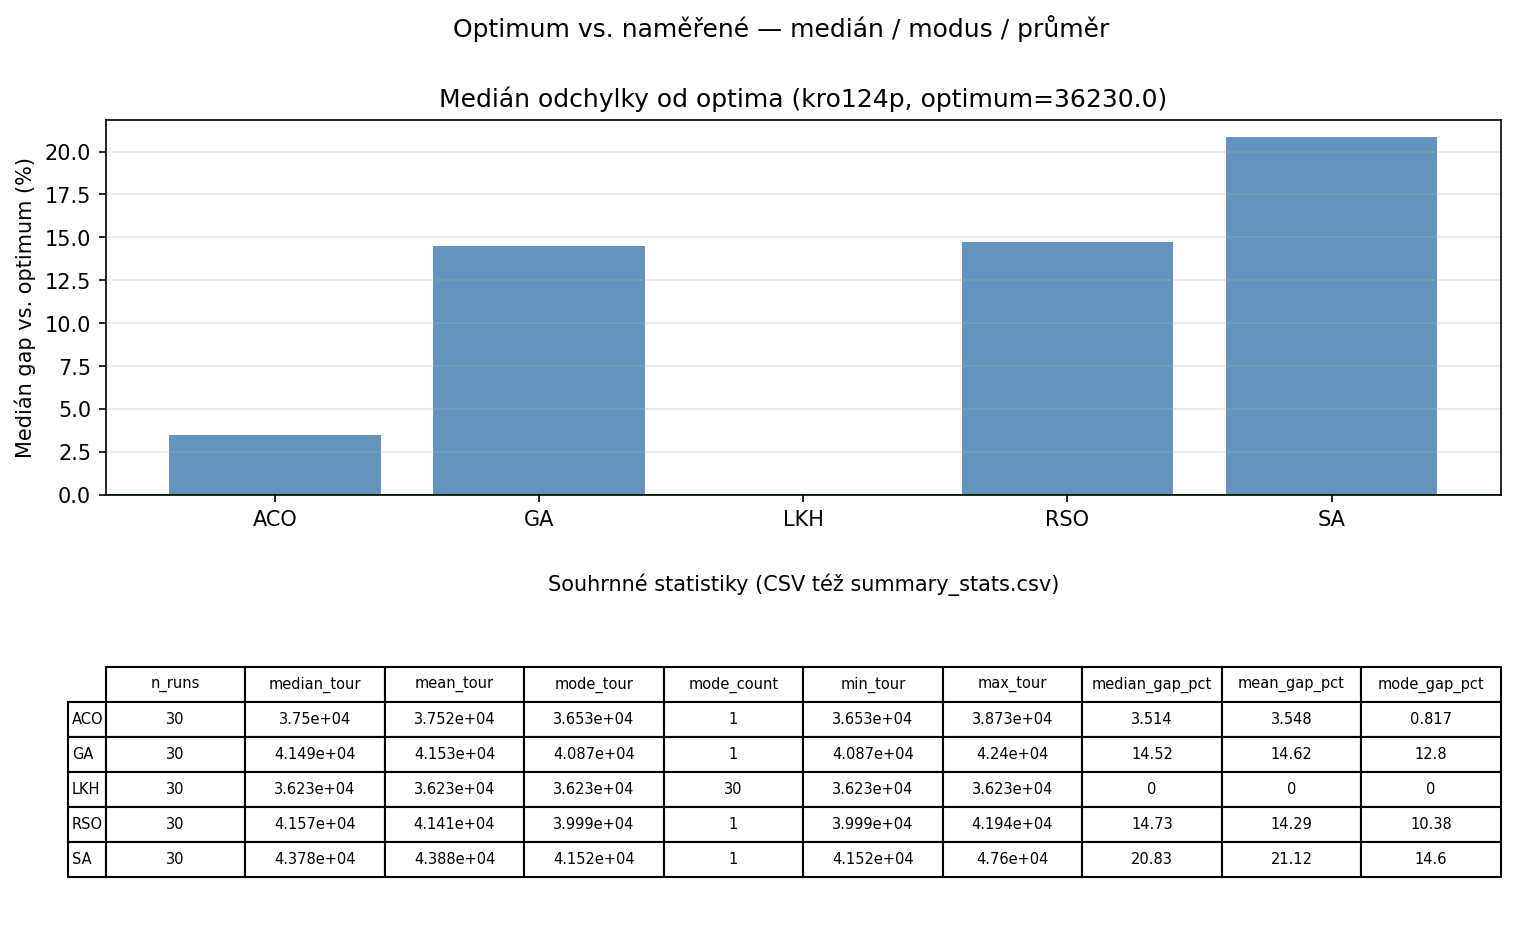
\includegraphics[width=\textwidth]{Figures/asymmetric_kro124p/summary_table_optimum_vs_stats.png}
    \caption{Souhrnná tabulka výsledků pro instanci \texttt{kro124p}}
    \label{fig:summary_table_optimum_vs_stats_kro124p}
\end{figure}

\section{Zhodnocení a omezení interpretace}
\label{sec:exp_limits}
Zařazení instancí \texttt{a280} a \texttt{kro124p} poskytuje robustnější pohled než vyhodnocení jediné úlohy, protože umožňuje sledovat chování metod v symetrickém i asymetrickém prostředí. Přesto je nutné výsledky interpretovat s ohledem na to, že jde stále o omezenou experimentální sadu a že relativní pořadí stochastických metod může být citlivé na konkrétní kombinaci instance a naladění parametrů.

Z praktického hlediska měření potvrzuje, že volba algoritmu musí vycházet z požadované rovnováhy mezi kvalitou a časem výpočtu a současně respektovat vlastnosti řešené úlohy. U asymetrických instancí je zejména důležité počítat s tím, že část klasických lokálních metod určených pro symetrický TSP není přímo použitelná a musí být nahrazena operátory navrženými pro orientované hrany.